\vspace{2mm}
\begin{figure}[h!]
\tikzset{every picture/.style={line width=0.75pt}} %set default line width to 0.75pt        

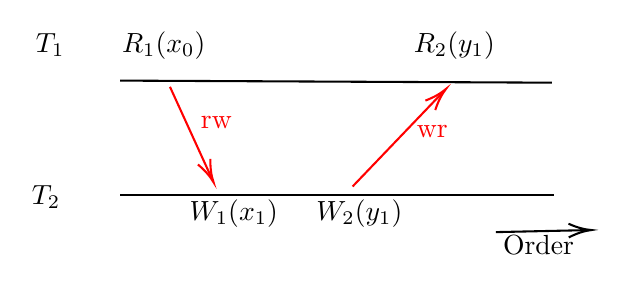
\begin{tikzpicture}[x=0.75pt,y=0.75pt,yscale=-1,xscale=1]
%uncomment if require: \path (0,300); %set diagram left start at 0, and has height of 300

%Straight Lines [id:da9500410641573396] 
\draw    (63.56,64) -- (271.56,65) ;
%Straight Lines [id:da7796185686481738] 
\draw    (63.56,119) -- (272.56,119) ;
%Straight Lines [id:da7329480179958066] 
\draw    (244.56,137) -- (288.56,136.04) ;
\draw [shift={(290.56,136)}, rotate = 178.75] [color={rgb, 255:red, 0; green, 0; blue, 0 }  ][line width=0.75]    (10.93,-3.29) .. controls (6.95,-1.4) and (3.31,-0.3) .. (0,0) .. controls (3.31,0.3) and (6.95,1.4) .. (10.93,3.29)   ;
%Straight Lines [id:da06917928011783969] 
\draw [color={rgb, 255:red, 255; green, 0; blue, 0 }  ,draw opacity=1 ]   (87.56,67) -- (107.73,111.18) ;
\draw [shift={(108.56,113)}, rotate = 245.46] [color={rgb, 255:red, 255; green, 0; blue, 0 }  ,draw opacity=1 ][line width=0.75]    (10.93,-3.29) .. controls (6.95,-1.4) and (3.31,-0.3) .. (0,0) .. controls (3.31,0.3) and (6.95,1.4) .. (10.93,3.29)   ;
%Straight Lines [id:da061796007668484476] 
\draw [color={rgb, 255:red, 255; green, 0; blue, 0 }  ,draw opacity=1 ]   (175.56,115) -- (219.18,69.44) ;
\draw [shift={(220.56,68)}, rotate = 133.75] [color={rgb, 255:red, 255; green, 0; blue, 0 }  ,draw opacity=1 ][line width=0.75]    (10.93,-3.29) .. controls (6.95,-1.4) and (3.31,-0.3) .. (0,0) .. controls (3.31,0.3) and (6.95,1.4) .. (10.93,3.29)   ;

% Text Node
\draw (21.5,40) node [anchor=north west][inner sep=0.75pt]   [align=left] {$T_1$};
% Text Node
\draw (19.5,113) node [anchor=north west][inner sep=0.75pt]   [align=left] {$T_2$};
% Text Node
\draw (156.56,120) node [anchor=north west][inner sep=0.75pt]   [align=left] {$W_2(y_1)$};
% Text Node
\draw (63,39) node [anchor=north west][inner sep=0.75pt]   [align=left] {$R_1(x_0)$};
% Text Node
\draw (246.56,137) node [anchor=north west][inner sep=0.75pt]   [align=left] {Order};
% Text Node
\draw (203.56,39) node [anchor=north west][inner sep=0.75pt]   [align=left] {$R_2(y_1)$};
% Text Node
\draw (95.56,120) node [anchor=north west][inner sep=0.75pt]   [align=left] {$W_1(x_1)$};
% Text Node
\draw (101,80) node [anchor=north west][inner sep=0.75pt]  [color={rgb, 255:red, 255; green, 0; blue, 0 }  ,opacity=1 ] [align=left] {rw};
% Text Node
\draw (205,84) node [anchor=north west][inner sep=0.75pt]  [color={rgb, 255:red, 255; green, 0; blue, 0 }  ,opacity=1 ] [align=left] {wr};


\end{tikzpicture}
    \caption{G-single cycle between $T_1$ and $T_2$, (rw, wr)}
\end{figure}
\vspace{2mm}
\begin{equation}
History\ H: [R_1(x_0),W_1(x_1),W_2(y_1),R_2(yx_1)]
\end{equation}
\vspace{2mm}